% PI-CON architecture diagram — TikZ vector source (matches the clean codex reference look).
% Package-free tight crop (TeX Live basic has no standalone/preview): ship a single \hbox
% sized page. Compile:  pdflatex architecture_src.tex  ->  architecture_src.pdf
\documentclass{article}
\usepackage{tikz}
\usepackage{amsmath}
\usetikzlibrary{arrows.meta,positioning,fit,backgrounds,calc}
\pagestyle{empty}

\definecolor{picon}{HTML}{0072B2}
\definecolor{piconfill}{HTML}{E9F2FB}
\definecolor{inkline}{HTML}{1A1A1A}
\definecolor{lanefill}{HTML}{F5F7F9}
\definecolor{laneedge}{HTML}{DDE4EA}

\newcommand{\ttl}[1]{\textbf{#1}}
\newcommand{\btl}[1]{\textcolor{picon}{\textbf{#1}}}
\newcommand{\sub}[1]{{\footnotesize #1}}

\begin{document}%
\setbox0=\hbox{%
\hyphenpenalty=10000\exhyphenpenalty=10000\relax
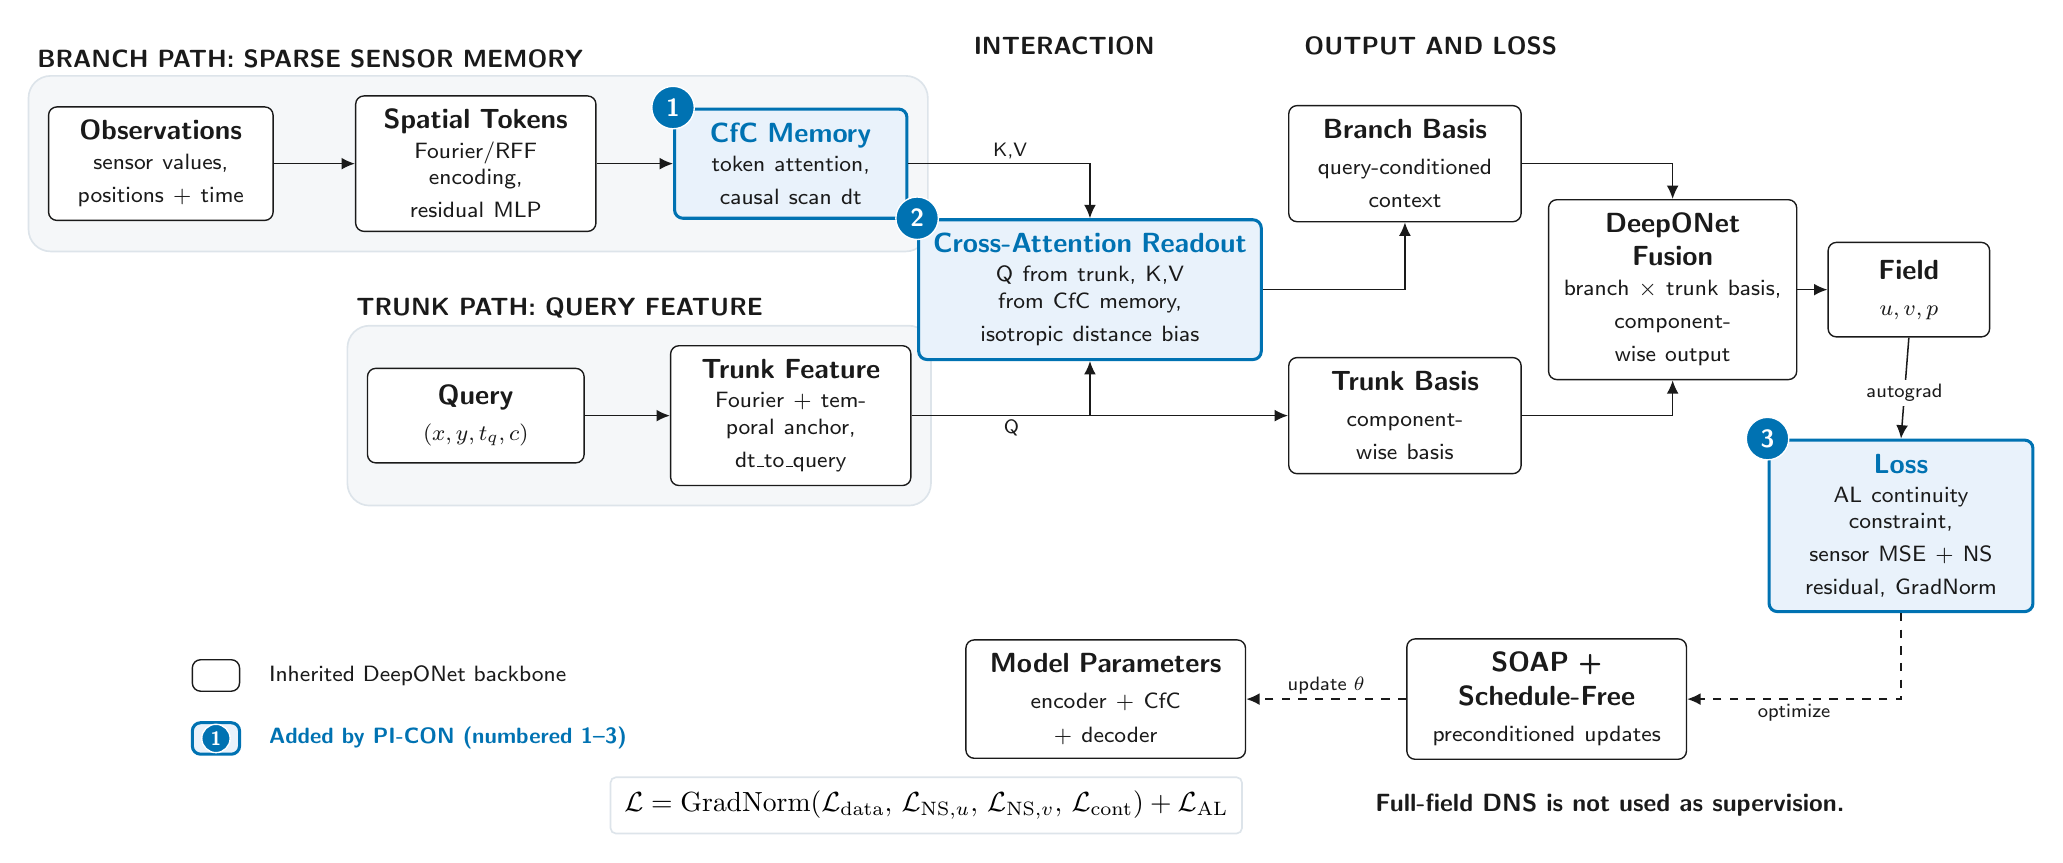
\begin{tikzpicture}[
  font=\sffamily,
  >={Latex[length=1.7mm,width=1.5mm]},
  box/.style={rounded corners=3pt, draw=inkline, line width=0.5pt, fill=white,
              align=center, inner sep=5pt, minimum height=1.2cm, text=inkline},
  picon/.style={rounded corners=3pt, draw=picon, line width=1.1pt, fill=piconfill,
                align=center, inner sep=5pt, minimum height=1.2cm, text=inkline},
  badge/.style={circle, fill=picon, text=white, inner sep=0pt, minimum size=5.4mm,
                font=\sffamily\bfseries\small, draw=white, line width=0.5pt},
  lane/.style={rounded corners=8pt, draw=laneedge, fill=lanefill, line width=0.6pt,
               inner sep=7pt},
  zone/.style={font=\sffamily\bfseries\small, text=inkline, anchor=west},
  arr/.style={->, draw=inkline, line width=0.55pt},
  darr/.style={->, draw=inkline, line width=0.55pt, dashed},
  elab/.style={font=\sffamily\scriptsize, text=inkline, inner sep=1.5pt, fill=white},
]

% ---- branch row ----
\node[box, text width=2.5cm]  (obs)  at (0,0)      {\ttl{Observations}\\[1pt]\sub{sensor values,\\ positions + time}};
\node[box, text width=2.7cm]  (spat) at (4.0,0)    {\ttl{Spatial Tokens}\\[1pt]\sub{Fourier/RFF encoding,\\ residual MLP}};
\node[picon, text width=2.6cm](cfc)  at (8.0,0)    {\btl{CfC Memory}\\[1pt]\sub{token attention,\\ causal scan dt}};

% ---- trunk row ----
\node[box, text width=2.4cm]  (qry)  at (4.0,-3.2) {\ttl{Query}\\[1pt]\sub{$(x,y,t_q,c)$}};
\node[box, text width=2.7cm]  (tf)   at (8.0,-3.2) {\ttl{Trunk Feature}\\[1pt]\sub{Fourier + temporal anchor,\\ dt\_to\_query}};

% ---- interaction ----
\node[picon, text width=4.0cm](ca)   at (11.8,-1.6){\btl{Cross-Attention Readout}\\[1pt]\sub{Q from trunk, K,V from CfC memory,\\ isotropic distance bias}};

% ---- output ----
\node[box, text width=2.6cm]  (bb)   at (15.8,0.0) {\ttl{Branch Basis}\\[1pt]\sub{query-conditioned context}};
\node[box, text width=2.6cm]  (tb)   at (15.8,-3.2){\ttl{Trunk Basis}\\[1pt]\sub{component-wise basis}};
\node[box, text width=2.8cm]  (fus)  at (19.2,-1.6){\ttl{DeepONet Fusion}\\[1pt]\sub{branch $\times$ trunk basis,\\ component-wise output}};
\node[box, text width=1.7cm]  (fld)  at (22.2,-1.6){\ttl{Field}\\[1pt]\sub{$u,v,p$}};
\node[picon, text width=3.0cm](loss) at (22.1,-4.6){\btl{Loss}\\[1pt]\sub{AL continuity constraint,\\ sensor MSE + NS residual, GradNorm}};

% ---- optimizer feedback ----
\node[box, text width=3.2cm]  (mp)   at (12.0,-6.8){\ttl{Model Parameters}\\[1pt]\sub{encoder + CfC + decoder}};
\node[box, text width=3.2cm]  (opt)  at (17.6,-6.8){\ttl{SOAP + Schedule-Free}\\[1pt]\sub{preconditioned updates}};

% ---- badges (straddle top-left corner) ----
\node[badge] at (cfc.north west)  {1};
\node[badge] at (ca.north west)   {2};
\node[badge] at (loss.north west) {3};

% ---- lanes (behind) + zone headers ----
\begin{scope}[on background layer]
  \node[lane, fit=(obs)(spat)(cfc)] (blane) {};
  \node[lane, fit=(qry)(tf)] (tlane) {};
\end{scope}
\node[zone] at ([yshift=6pt]blane.north west) {BRANCH PATH: SPARSE SENSOR MEMORY};
\node[zone] at ([yshift=6pt]tlane.north west) {TRUNK PATH: QUERY FEATURE};
\node[zone] at (10.2,1.5) {INTERACTION};
\node[zone] at (14.4,1.5) {OUTPUT AND LOSS};

% ---- arrows ----
\draw[arr] (obs) -- (spat);
\draw[arr] (spat) -- (cfc);
\draw[arr] (cfc.east) -| (ca.north) node[elab, pos=0.28, above] {K,V};
\draw[arr] (qry) -- (tf);
\draw[arr] (tf.east) -| (ca.south) node[elab, pos=0.28, below] {Q};
\draw[arr] (tf.east) -- (tb.west);
\draw[arr] (ca.east) -| (bb.south);
\draw[arr] (bb.east) -| (fus.north);
\draw[arr] (tb.east) -| (fus.south);
\draw[arr] (fus) -- (fld);
\draw[arr] (fld.south) -- (loss.north) node[elab, pos=0.55] {autograd};
\draw[darr] (loss.south) |- (opt.east) node[elab, pos=0.75, below] {optimize};
\draw[darr] (opt) -- (mp) node[elab, midway, above] {update $\theta$};

% ---- legend ----
\node[box, minimum width=6mm, minimum height=4mm, text width=0pt, inner sep=0pt] (lg1) at (0.7,-6.5) {};
\node[font=\sffamily\footnotesize, anchor=west, text=inkline] at (1.25,-6.5) {Inherited DeepONet backbone};
\node[picon, minimum width=6mm, minimum height=4mm, text width=0pt, inner sep=0pt] (lg2) at (0.7,-7.3) {};
\node[badge, minimum size=3.6mm, font=\sffamily\bfseries\scriptsize] at (lg2.center) {1};
\node[font=\sffamily\footnotesize, anchor=west, text=picon] at (1.25,-7.3) {\bfseries Added by PI-CON (numbered 1--3)};

% ---- loss formula (native LaTeX math) + supervision note ----
\node[draw=laneedge, rounded corners=2pt, fill=white, line width=0.6pt, inner sep=5pt, anchor=west]
  at (5.7,-8.15) {$\mathcal{L} = \mathrm{GradNorm}\!\left(\mathcal{L}_{\mathrm{data}},\,
    \mathcal{L}_{\mathrm{NS},u},\, \mathcal{L}_{\mathrm{NS},v},\, \mathcal{L}_{\mathrm{cont}}\right)
    + \mathcal{L}_{\mathrm{AL}}$};
\node[font=\sffamily\bfseries\small, text=inkline, anchor=west] at (15.3,-8.15) {Full-field DNS is not used as supervision.};

\end{tikzpicture}%
}%
\pdfpagewidth=\wd0
\pdfpageheight=\dimexpr\ht0+\dp0\relax
\hoffset=-1in \voffset=-1in
\shipout\box0
\end{document}
